\documentclass[sigconf,balance=false]{acmart}
\usepackage{popets}

% Copyright
\setcopyright{popets}
\copyrightyear{2027}

% Issue info
\acmYear{2027}
\acmVolume{2027}
\acmNumber{1}
\acmDOI{XXXXXXX.XXXXXXX}
\acmISBN{}
\acmConference{Proceedings on Privacy Enhancing Technologies}
\settopmatter{printacmref=false,printccs=false,printfolios=true}

\usepackage{graphicx}
\usepackage{booktabs}
\usepackage{amsmath}
\usepackage{xcolor}
\usepackage{multirow}

\begin{document}

\title[Topic-Bottleneck Query Reformulation]{Topic-Bottleneck Query Reformulation for Privacy-Preserving Cloud LLM Inference}

\author{Andreas Tonio Liebrand}
\affiliation{%
  \institution{}
  \country{}}

\begin{abstract}
We introduce \emph{topic-bottleneck query reformulation}, a pipeline for privacy-preserving inference with cloud-hosted large language models (LLMs) that routes sensitive enterprise queries through an irreversible information bottleneck.
Unlike entity substitution and differential privacy (DP) methods---from which modern LLMs recover 72--94\% of original sensitive content---our approach compresses a sensitive query into a topic distribution via a local model, generates generic proxy questions from that distribution, and sends only these questions---which contain no sensitive specifics by construction---to the cloud.
A local model then synthesizes the final answer by applying the cloud-obtained reasoning frameworks to the locally-held sensitive context.
Evaluated on 48 answerable contract QA pairs from the CUAD dataset, the pipeline achieves a \textbf{2.3\% specific value recovery rate} (compared to 91--94\% for DP methods) while preserving \textbf{89.3\% BERTScore F1} relative to an oracle with full access to the sensitive query.
An optional vocabulary exclusion hardening layer reduces recovery to 0\% at the cost of a 7-percentage-point BERTScore reduction.
We characterize the pipeline's operating envelope across four task types: framework/reasoning, compliance, and procedural queries achieve zero recovery with strong quality, while entity-specific queries exhibit the expected quality-privacy trade-off.
We openly discuss the absence fingerprint vulnerability introduced by vocabulary exclusion and propose four mitigations.
\end{abstract}

\keywords{privacy-preserving inference, large language models, topic modeling, information bottleneck, differential privacy, query reformulation}

\maketitle

%% ============================================================
%% SECTION 1: INTRODUCTION
%% ============================================================
\section{Introduction}
\label{sec:intro}

State-of-the-art large language models (LLMs)---GPT-4o, Claude, Gemini---are available exclusively through cloud APIs operated by a small number of providers.
Their utility for enterprise applications scales with the specificity of the input: the more contextual detail a prompt contains, the more targeted and valuable the response.
Yet enterprises holding classified data---merger and acquisition strategies, financial projections, health records, competitive intelligence---face hard legal constraints that prohibit transmitting such data to cloud providers.
GDPR Article~5(1)(c) mandates data minimization; HIPAA requires de-identification of protected health information; and the US CLOUD Act empowers US authorities to compel US-incorporated cloud providers to disclose data regardless of its physical storage location, including data hosted in EU data centers.

This creates a fundamental tension: \emph{LLM value is proportional to prompt specificity, but privacy requires removing specificity before transmission.}
Every existing approach to resolving this tension attempts to preserve specificity while hiding identity---and fails, because modern LLMs can reverse the hiding.
Entity substitution methods~\cite{chen2023, albanese2026, agyemang2026, yang2025} replace sensitive entities with pseudonyms, creating a one-to-one mapping that is structurally invertible.
Differential privacy (DP) methods~\cite{yue2021, chen2023custext, tem2021, cape2025, inferdpt2023, dyntext2025, clusant2025} add calibrated noise to token embeddings, but Pang et al.~\cite{pang2024} demonstrated that modern LLMs recover 72--94\% of original sensitive content from DP-sanitized text, with Claude-3.5 Sonnet achieving 94.01\% recovery.
This reconstruction attack fundamentally limits all approaches that transmit a modified version of the sensitive content.

We propose a qualitatively different mechanism: \emph{topic-bottleneck query reformulation}.
Rather than sanitizing a sensitive prompt by modifying its tokens, we compress it through a \emph{many-to-one} semantic bottleneck---topic modeling---that strips sensitive specifics while preserving reasoning structure.
An enormous number of different sensitive prompts map to the same topic distribution; exact reconstruction from the distribution is infeasible---bounded by the bottleneck's information capacity rather than a statistical privacy budget.
The pipeline generates generic proxy questions from the topic distribution, sends only these to the cloud LLM, and synthesizes the final answer locally by applying the cloud-obtained reasoning frameworks to the locally-held sensitive context.

\paragraph{Contributions.} We make four contributions:

\begin{enumerate}
\item \textbf{Topic modeling as an irreversible privacy bottleneck.} We formalize topic extraction as a many-to-one information bottleneck for privacy-preserving LLM inference. Unlike entity substitution (one-to-one) and DP noise (many-to-many within a recoverable neighborhood), many-to-one compression is structurally irreversible.

\item \textbf{Vocabulary exclusion hardening.} We introduce a novel second compression layer that strips domain vocabulary from the generated text before proxy question creation. When combined with the topic bottleneck, the cloud LLM receives neither the original content nor the lexical anchors that would enable re-identification. To our knowledge, this technique has not appeared in the existing literature.

\item \textbf{Local synthesis architecture.} We demonstrate that a local LLM can apply externally-obtained, generic reasoning frameworks to locally-held sensitive specifics---analogous to how a consultant looks up best practices externally and applies them to a confidential internal situation.

\item \textbf{Empirical operating envelope characterization.} We provide honest, task-type-level characterization of where the pipeline works and where it degrades, evaluated on the CUAD dataset: 2.3\% specific value recovery (vs.\ 91--94\% for DP), 89.3\% BERTScore F1, with zero recovery for framework, compliance, and procedural queries and 9.2\% for entity-specific queries.
\end{enumerate}

%% ============================================================
%% SECTION 2: RELATED WORK
%% ============================================================
\section{Related Work}
\label{sec:related}

We organize prior work into four families that span the landscape of privacy-preserving LLM inference.

\subsection{Prompt Sanitization and Entity Substitution}
\label{sec:rw-entity}

The most widely deployed family detects sensitive entities via named entity recognition (NER) and replaces them with pseudonyms or abstractions before sending the sanitized prompt to a cloud LLM.
Chen et al.~\cite{chen2023} propose Hide and Seek (HaS), a two-stage framework where a ``Hide'' step anonymizes private entities and a locally-trained ``Seek'' model de-anonymizes the returned results.
CON-QA~\cite{conqa2025} extends this to contract-domain QA with one-to-many anonymization mappings that prevent cross-session entity inference, achieving 98.8\% entity restoration accuracy.
Albanese et al.~\cite{albanese2026} introduce Anonymous-by-Construction, a fully on-premise pipeline that replaces PII with realistic, type-consistent surrogates.
RUPTA~\cite{yang2025} explicitly defends against LLM-based re-identification attacks, demonstrating that classical anonymization methods are insufficient when the adversary can reason over dispersed contextual patterns.
LLM-Redactor~\cite{agyemang2026} benchmarks eight anonymization techniques on 1,300 labeled samples, finding that no single technique dominates and that combined approaches achieve 0.6\% PII leak at the cost of 31.3\% proprietary code leak.

All entity substitution methods share a structural limitation: they maintain a bijective or near-bijective mapping between the original and sanitized text. Our approach avoids entity-level processing entirely, instead compressing through a many-to-one semantic bottleneck.

\subsection{Differential Privacy for Text}
\label{sec:rw-dp}

Token-level differential privacy methods apply calibrated noise to word embeddings before transmission, providing formal privacy guarantees parameterized by~$\varepsilon$.
Foundational methods include SanText~\cite{yue2021}, CusText~\cite{chen2023custext}, and TEM~\cite{tem2021}.
Recent advances include CAPE~\cite{cape2025}, which integrates contextual information with token embedding distances via a hybrid utility function at ICML~2025; InferDPT~\cite{inferdpt2023}, which achieves quality comparable to non-private GPT-4 at $\varepsilon = 6.0$; DYNTEXT~\cite{dyntext2025}, which adapts protection level to semantic context; and CluSanT~\cite{clusant2025}, which unifies prior methods as special cases.
Chowdhury et al.~\cite{chowdhury2025} propose Pr$\varepsilon\varepsilon$mpt, a hybrid approach using format-preserving encryption for structured tokens and metric differential privacy for value-dependent tokens.

The critical limitation of all DP text methods was exposed by Pang et al.~\cite{pang2024}, who demonstrated that modern LLMs can reconstruct DP-sanitized text with recovery rates of 72.18\% (LLaMA-2 70B), 82.39\% (LLaMA-3 70B), 75.35\% (Gemma-2), 91.2\% (GPT-4o), and 94.01\% (Claude-3.5 Sonnet).
The mechanism is that LLMs memorize broad training data distributions, and DP-sanitized text falls within the support of those distributions, enabling in-context learning to bridge the gap.
This vulnerability worsens as models improve, making pure DP insufficient for high-stakes data.

Unlike DP methods, which transmit a perturbed version of the original text (leaving recoverable traces), our pipeline transmits independently generated proxy questions derived from topic distributions, with no bijective mapping to the original.

\subsection{Hybrid Cloud-Edge and Split Inference}
\label{sec:rw-split}

Architectural approaches partition inference across trust boundaries.
Split-and-Denoise (SnD)~\cite{snd2023} runs the token embedding layer locally and adds LDP noise to embeddings before transmission.
PRISM~\cite{zhan2025} implements a four-stage cloud-edge framework with entity-level sensitivity profiling and two-layer LDP, achieving 40--50\% energy and latency reduction.
Trusted Execution Environments (TEEs) provide hardware-level guarantees: Chrapek et al.~\cite{chrapek2025} demonstrate less than 10\% throughput overhead on Intel TDX/SGX and 4--8\% on NVIDIA H100 Confidential Compute.
Fully homomorphic encryption (FHE) offers the strongest theoretical guarantees but remains impractical: EncryptedLLM~\cite{decastro2025} achieves a 200$\times$ GPU speedup over CPU baselines but is still limited to GPT-2-scale models; PermLLM~\cite{zheng2024} achieves approximately 3 seconds per token for ChatGLM-6B.

These approaches require either specialized hardware (TEE, FHE) or model modifications (split inference).
Our pipeline requires only a local small language model and a cloud API---no specialized hardware, no model modifications, and no cryptographic protocols.
Privacy is achieved through information-theoretic compression rather than computational hardness assumptions.

\subsection{Data Minimization and Privacy Metrics}
\label{sec:rw-minimization}

Zhou et al.~\cite{zhou2025} demonstrate that GPT-4-class models tolerate 85.7\% information redaction while maintaining task performance, revealing that the practical sanitization floor is much lower than intuition suggests.
Carpentier et al.~\cite{carpentier2024} propose a middleware SLM that predicts whether a DP-sanitized prompt will produce poor output, preventing resource waste for up to 20\% of prompts.
Privacy-preserving RAG~\cite{zeng2024, syntheticrag2024, dprag2024} addresses corpus-level privacy but not prompt-level privacy.

A comprehensive survey of text anonymization metrics~\cite{metricssurvey2025} reviews 47~papers across six distinct privacy notions and finds that existing metrics ``often fail to fully capture legal standards and user expectations''---GDPR and HIPAA compliance cannot be certified by any current anonymization metric alone.

Our approach operationalizes data minimization at the semantic level: the topic bottleneck transmits only the minimum information needed (topic structure) while ensuring that all sensitive specifics are irreversibly compressed away.

%% ============================================================
%% SECTION 3: THREAT MODEL AND PROBLEM FORMULATION
%% ============================================================
\section{Threat Model and Problem Formulation}
\label{sec:threat}

\subsection{Sensitivity Classification}
\label{sec:sensitivity}

We adopt a four-level sensitivity taxonomy that maps to regulatory requirements:

\begin{itemize}
\item \textbf{S0 (Public):} Press releases, public filings, general knowledge. May freely leave the organization.
\item \textbf{S1 (Confidential):} Internal processes, organizational charts, product roadmaps. May not leave the organization.
\item \textbf{S2 (Highly Confidential):} Merger/acquisition plans, financial projections, competitive intelligence. Breach entails material legal risk. Subject to GDPR data minimization requirements.
\item \textbf{S3 (Strictly Confidential):} Health records, personal data under GDPR/HIPAA. Breach entails regulatory liability. Subject to HIPAA de-identification standards.
\end{itemize}

The pipeline targets S1--S3 queries where the user seeks cloud LLM reasoning capability but cannot transmit the query's sensitive content.

\subsection{Adversary Model}
\label{sec:adversary}

\paragraph{Adversary.} The cloud LLM provider, or any party with access to the data transmitted to the cloud. The adversary has full access to the S0 proxy questions sent via the API and possesses state-of-the-art LLM capabilities for reconstruction attacks. We follow the attack methodology of Pang et al.~\cite{pang2024}: the adversary attempts to reconstruct the original sensitive content from the transmitted content using direct prompting and domain-expert prompting.

\paragraph{What is protected.} Specific entity names, numerical values (deal sizes, financial figures, patient identifiers), temporal references, and any content classified S1 or above.

\paragraph{What is not protected.} The general domain or topic of the query. We explicitly accept that an adversary can determine that the user is asking about, e.g., corporate acquisitions or contract compliance. Domain recovery is intentional: the topic structure must be preserved for the proxy questions to elicit useful reasoning from the cloud LLM. The privacy claim is that the adversary cannot recover the \emph{specific} sensitive details---who, how much, when---even with knowledge of the general domain.

%% ============================================================
%% SECTION 4: METHODOLOGY
%% ============================================================
\section{Methodology}
\label{sec:method}

\subsection{Pipeline Overview}
\label{sec:pipeline-overview}

The pipeline comprises six steps executed across a trust boundary between a local environment (trusted, holds the sensitive S2/S3 query) and a cloud LLM (untrusted, receives only S0 content). Figure~\ref{fig:pipeline} provides a visual overview. Let $q_s$ denote the original sensitive query (S2 or S3), and let $\mathcal{M}_L$ and $\mathcal{M}_C$ denote the local and cloud LLMs, respectively.

\begin{figure*}[t]
\centering
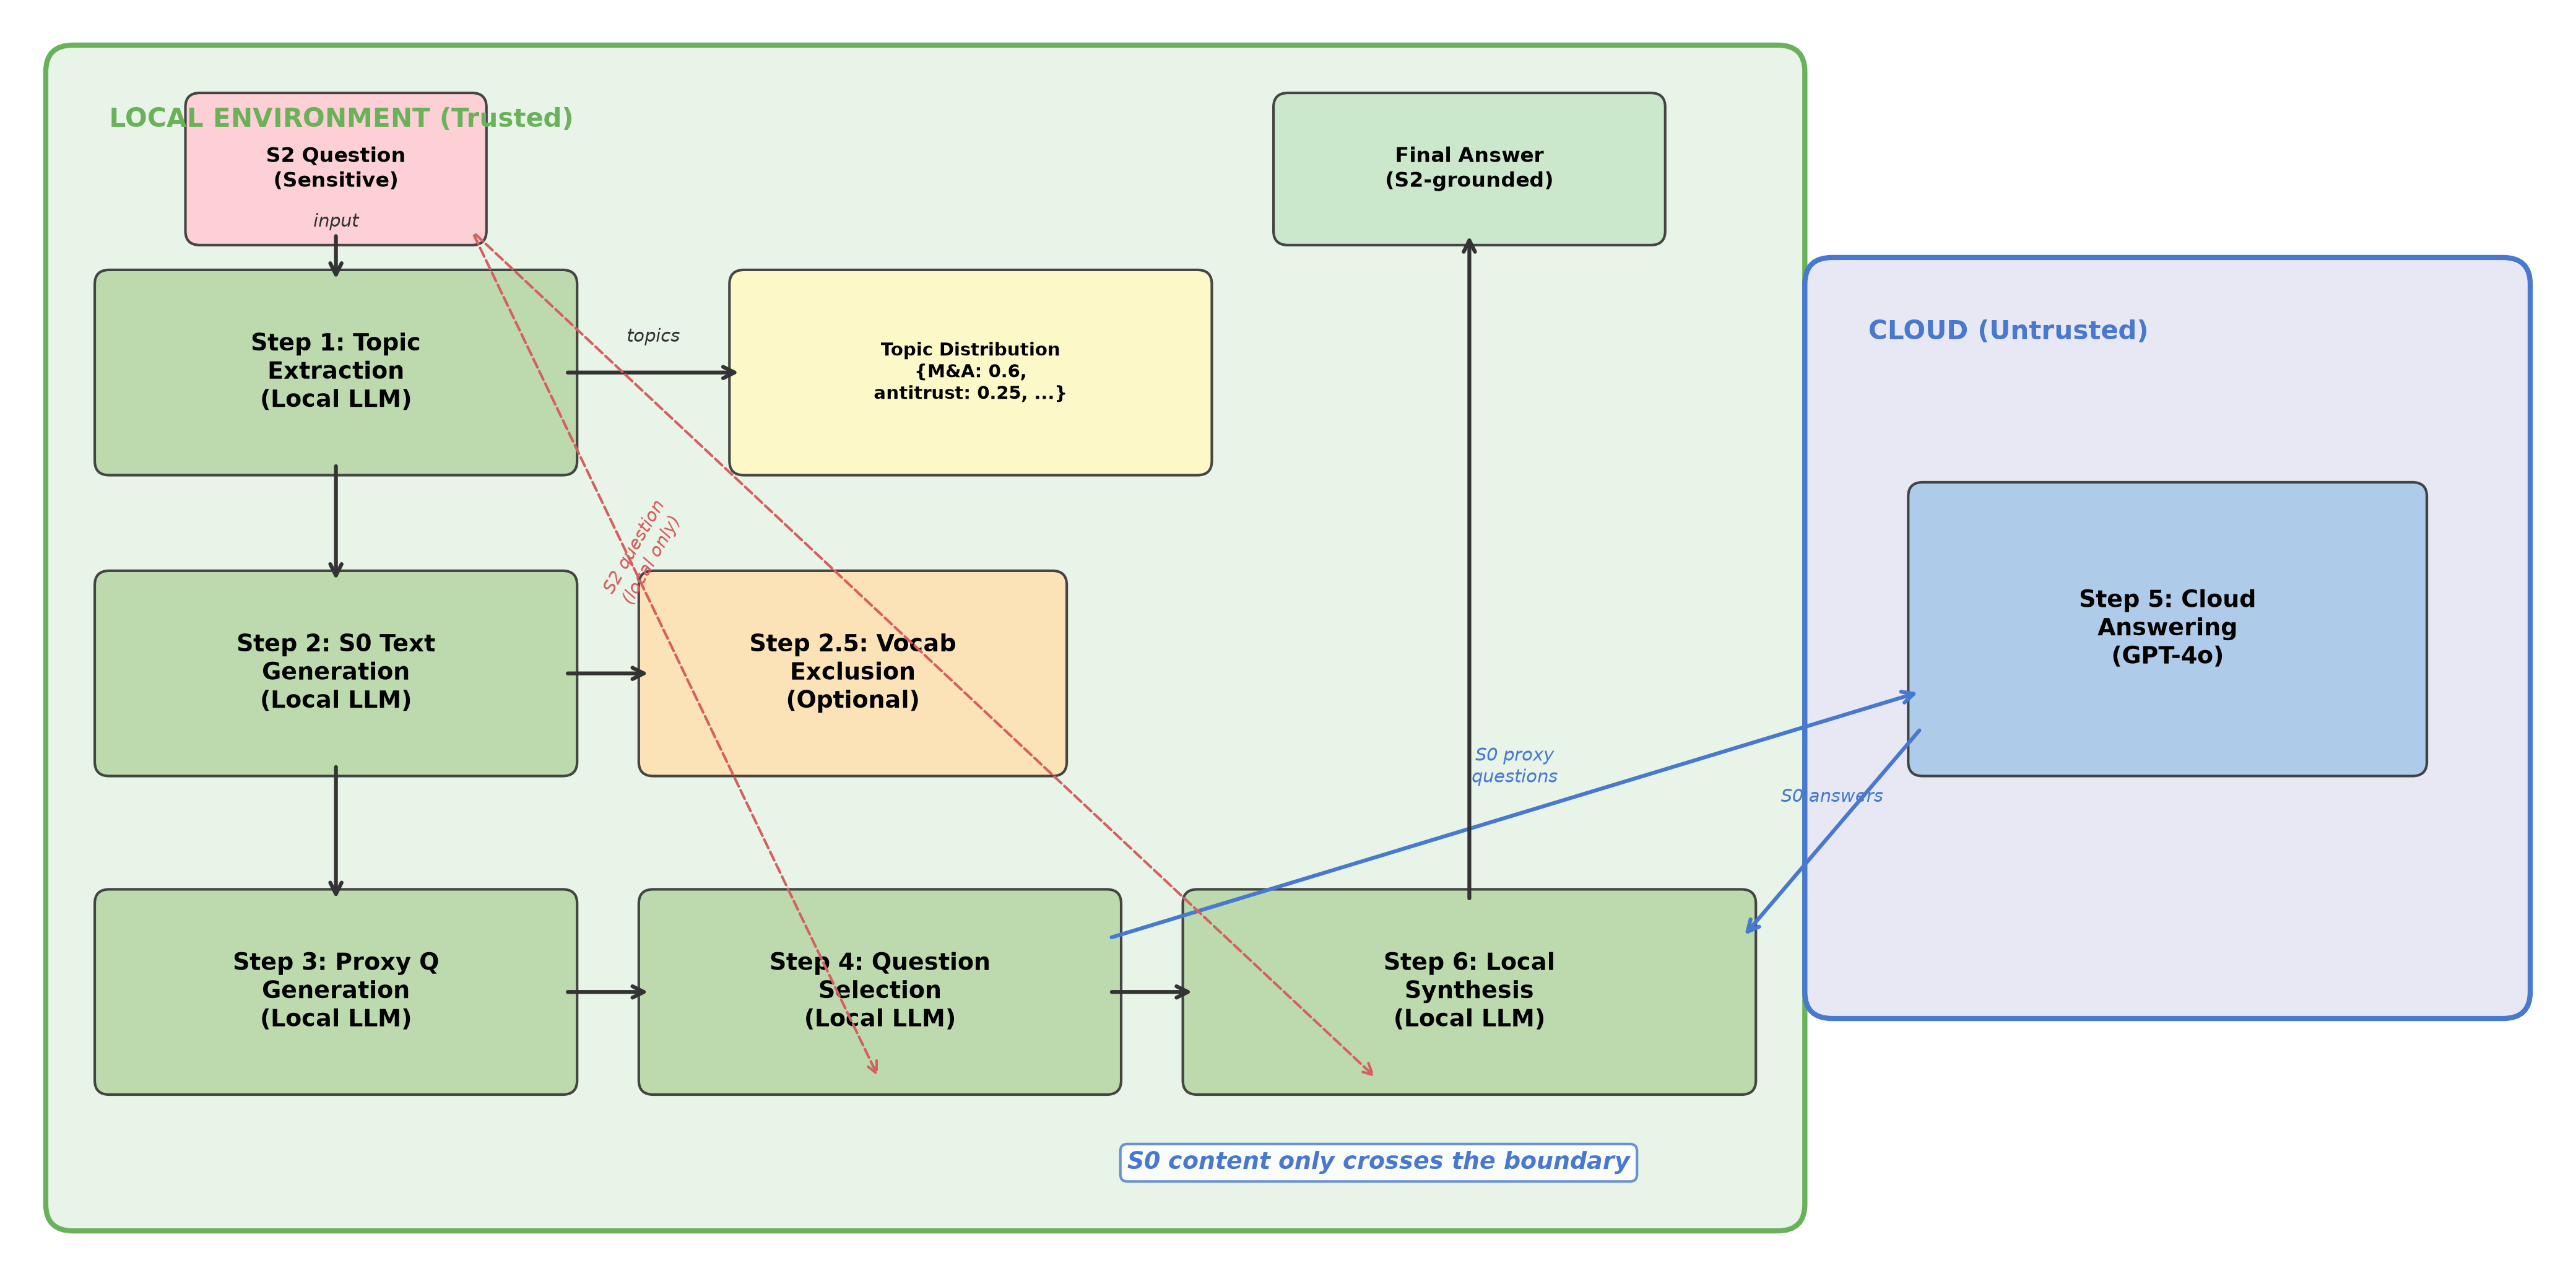
\includegraphics[width=0.85\textwidth]{fig_pipeline_architecture.png}
\caption{Overview of the topic-bottleneck query reformulation pipeline. The six-step process extracts a topic distribution from a sensitive (S2) question, generates generic S0 text, optionally applies vocabulary exclusion, generates and selects proxy questions, sends only S0 content to the cloud LLM, and synthesizes the final answer locally. Dashed red arrows indicate paths where the S2 question is used only locally. The trust boundary separates the local environment (green) from the cloud (blue).}
\label{fig:pipeline}
\end{figure*}

\subsection{Topic Extraction and S0 Text Generation}
\label{sec:topic-extraction}

\paragraph{Step 1: Topic Extraction.} The local LLM $\mathcal{M}_L$ extracts a topic distribution $\boldsymbol{\tau} = \{(t_i, w_i)\}_{i=1}^{k}$ from the sensitive query $q_s$, where $t_i$ is a topic label and $w_i \in [0, 1]$ is its weight, with $\sum_i w_i = 1$. For example, the query ``Should we acquire TechCorp at EUR~2.3B given their 60\% EU market share?'' yields:
\[
\boldsymbol{\tau} = \bigl\{(\text{M\&A},\, 0.6),\; (\text{antitrust},\, 0.25),\; (\text{ent.\ SaaS},\, 0.15)\bigr\}
\]

This step implements a \emph{many-to-one compression}: an enormous number of different sensitive queries---involving different companies, deal sizes, market shares, and timelines---map to the same topic distribution. The compression is irreversible by design: one cannot reconstruct ``TechCorp, EUR~2.3B, 60\% EU market share'' from the topic distribution above.

\paragraph{Step 2: S0 Text Generation.} $\mathcal{M}_L$ generates 200--300 words of generic, factual, S0-level text about the topics in $\boldsymbol{\tau}$. This text contains no reference to the original query's specifics---it discusses the topic space in general terms. The text serves as the substrate from which proxy questions will be derived.

The key property distinguishing this from DP-based approaches is the nature of the transformation. DP applies a many-to-many perturbation within a recoverable neighborhood of the original text. Entity substitution creates a one-to-one mapping. Topic-based compression is many-to-one: the mapping from sensitive queries to topic distributions is a surjection with no inverse.

\subsection{Vocabulary Exclusion Hardening}
\label{sec:vocab-exclusion}

\paragraph{Step 2.5: Vocabulary Exclusion (Optional).} Before proxy question generation, all words from the topic vocabulary $V_\tau = \bigcup_i \text{vocab}(t_i)$ are stripped from the generated S0 text. This adds a second layer of many-to-one compression: the cloud LLM sees neither the original content nor the vocabulary that would anchor a topic-to-instance mapping.

For example, with topics $\{$M\&A, antitrust, SaaS$\}$, the exclusion set includes words like ``acquisition,'' ``merger,'' ``antitrust,'' ``EBITDA,'' and ``SaaS.'' After exclusion, ``In software M\&A, antitrust regulators examine market concentration'' becomes ``In strategic consolidation, regulators examine dominance metrics.''

\paragraph{Absence Fingerprint Vulnerability.} Vocabulary exclusion introduces a second-order information leak. An adversary who infers the general topic of the S0 text can compare the observed vocabulary against the vocabulary expected for that topic. Words that are conspicuously absent---``EBITDA,'' ``valuation,'' ``multiple''---form an \emph{absence fingerprint} that reveals which terms were stripped. The current implementation uses deterministic regex-based exclusion, making this fingerprint fully recoverable by an adversary with topic knowledge.

We identify four mitigations: (1)~random over-exclusion with decoy terms; (2)~paraphrase-based replacement instead of deletion; (3)~generation-time avoidance, where Step~2 is instructed to never produce topic-specific vocabulary (recommended default); (4)~fixed-size vocabulary masking from a predefined domain lexicon. The generation-time avoidance approach eliminates the attack surface entirely because no gap artifacts are created. We did not empirically evaluate these mitigations in the current study; this is left for future work (Section~\ref{sec:future}).

\subsection{Proxy Question Generation and Selection}
\label{sec:proxy-questions}

\paragraph{Step 3: Proxy Question Generation.} $\mathcal{M}_L$ generates $n = 10$ candidate S0 proxy questions from the (optionally vocabulary-stripped) S0 text. These questions cover the topic space broadly---e.g., ``What EBITDA multiples are typical for SaaS acquisitions?'' and ``How is antitrust risk assessed for dominant European tech players?''

\paragraph{Step 4: Question Selection.} $\mathcal{M}_L$ compares the original sensitive query $q_s$ against the $n$ candidates and selects the $k = 3$ most relevant proxy questions $\{p_1, p_2, p_3\}$. The selection criterion is semantic relevance as judged by $\mathcal{M}_L$. \emph{The original query $q_s$ is seen only by $\mathcal{M}_L$ in this step---it never leaves the local environment.}

\subsection{Cloud Answering and Local Synthesis}
\label{sec:synthesis}

\paragraph{Step 5: Cloud Answering.} The $k = 3$ selected S0 proxy questions are sent to the cloud LLM $\mathcal{M}_C$. The cloud receives genuinely S0 content---no sensitive data crosses the trust boundary. The cloud returns answers $\{a_1, a_2, a_3\}$.

\paragraph{Step 6: Local Synthesis.} $\mathcal{M}_L$ combines the original sensitive query $q_s$ with the three cloud-obtained S0 answers to produce the final answer~$a_f$. This mirrors how a consultant works: look up best practices externally (cloud LLM answers generic questions), apply them to a confidential internal situation (local LLM synthesizes with sensitive context). The synthesis step bridges S0 reasoning frameworks with S2/S3 specifics without ever transmitting the specifics.

\subsection{Privacy Analysis}
\label{sec:privacy-analysis}

We characterize the privacy properties of the topic bottleneck through the lens of the anonymity set and an upper bound on information leakage.

\paragraph{Anonymity set.} Let $\mathcal{Q}$ denote the space of all possible sensitive queries, and let $\tau: \mathcal{Q} \to \Delta^k$ be the topic extraction function mapping queries to $k$-topic distributions. The \emph{anonymity set} for a transmitted topic distribution $\boldsymbol{\tau}_0$ is $\mathcal{A}(\boldsymbol{\tau}_0) = \{q \in \mathcal{Q} : \tau(q) = \boldsymbol{\tau}_0\}$. An adversary who observes the proxy questions (which are derived solely from $\boldsymbol{\tau}_0$) cannot distinguish between any members of $\mathcal{A}(\boldsymbol{\tau}_0)$. For coarse topic distributions (e.g., $k = 3$ topics), the anonymity set is combinatorially large: any combination of entities, values, and dates within the same topic domain maps to the same distribution.

\paragraph{Information leakage bound.} The mutual information between the sensitive query $q_s$ and the transmitted proxy questions $P = \{p_1, \ldots, p_k\}$ is bounded by the information content of the intermediate topic distribution:
\[
I(q_s; P) \leq I(q_s; \boldsymbol{\tau}) \leq H(\boldsymbol{\tau})
\]
where $H(\boldsymbol{\tau})$ is the entropy of the topic distribution. Since $\boldsymbol{\tau}$ is a $k$-dimensional probability vector with typically $k \in [3, 6]$, this bounds information leakage to at most $\log_2(k!)$ bits for a uniform distribution over topic orderings---far less than the information content of the original query, which may contain hundreds of bits of specific entity, value, and temporal information. The topic bottleneck thus provides a \emph{structural} information bound, not a statistical one: leakage is bounded by the bottleneck's capacity, not by a privacy budget parameter.

\paragraph{Limitations of this analysis.} This bound assumes the topic extraction function is deterministic and that the proxy questions are conditionally independent of $q_s$ given $\boldsymbol{\tau}$. In practice, the local LLM's question selection step (Step~4) compares candidates against $q_s$ directly, which could introduce subtle correlations between $P$ and $q_s$ beyond what $\boldsymbol{\tau}$ captures. We leave a tighter analysis incorporating the selection step to future work.

%% ============================================================
%% SECTION 5: EXPERIMENTAL SETUP
%% ============================================================
\section{Experimental Setup}
\label{sec:setup}

\subsection{Dataset and Task Types}
\label{sec:dataset}

We evaluate on the CUAD (Contract Understanding Atticus Dataset) development split, selecting 48 answerable legal contract question-answer pairs. CUAD is a standard benchmark for contract analysis that contains enterprise-sensitive content (party names, monetary values, contractual terms) representative of S2-level data.

We categorize the 48~samples into four task types of 12~samples each, based on the nature of the query:

\begin{itemize}
\item \textbf{Framework/Reasoning} (n=12): Queries requiring analytical frameworks or reasoning structures (e.g., ``What are the key considerations for this type of agreement?'').
\item \textbf{Compliance/Regulatory} (n=12): Queries about regulatory obligations or compliance requirements.
\item \textbf{Procedural} (n=12): Queries about processes, steps, or procedural requirements.
\item \textbf{Entity-Specific} (n=12): Queries requiring specific entity names, values, or dates from the contract.
\end{itemize}

\subsection{Models and Configuration}
\label{sec:models}

The local LLM ($\mathcal{M}_L$) is Phi-3 (Microsoft), a 3.8B-parameter model suitable for on-premise deployment.
The cloud LLM ($\mathcal{M}_C$) is GPT-4o accessed via Azure OpenAI.
For each sample, the pipeline generates $n = 10$ proxy questions and selects $k = 3$ using LLM-based selection.

We run two configurations:
\begin{itemize}
\item \textbf{Baseline:} Vocabulary exclusion disabled (Step 2.5 skipped).
\item \textbf{Hardened:} Vocabulary exclusion enabled.
\end{itemize}

\subsection{Metrics and Baselines}
\label{sec:metrics}

\paragraph{Privacy metrics.}
\begin{itemize}
\item \textbf{Specific value recovery rate (SVR):} Our primary privacy metric. For each sample, the CUAD dataset provides a list of gold answer spans---the specific sensitive values the contract question targets (entity names, monetary amounts, dates, clause text). We give the adversary (GPT-4o) only the transmitted S0 proxy questions and ask it to reconstruct the original sensitive content. SVR is then the fraction of gold spans whose first 50 characters appear as case-insensitive substrings in the adversary's reconstruction: $\text{SVR} = \frac{|\{a \in A_\text{gold} : a[:50] \subseteq r\}|}{|A_\text{gold}|}$, where $r$ is the adversary's reconstruction. This is a strict, automated, exact-match criterion---semantic paraphrases do not count as recovery.
\item \textbf{Domain recovery rate:} Whether the adversary's reconstruction contains any content words ($>$3 characters) from the CUAD clause category label (e.g., ``change of control,'' ``non-compete'').
\item \textbf{Situation score:} Cosine similarity between sentence embeddings of the adversary's reconstruction and the first 500 characters of the original contract context, using the all-MiniLM-L6-v2 model. Ranges from 0 (unrelated) to 1 (identical).
\end{itemize}

\paragraph{Quality metrics.}
\begin{itemize}
\item \textbf{BERTScore F1:} Semantic similarity between the pipeline's answer and the oracle answer (cloud LLM given the full S2 question directly).
\item \textbf{Semantic similarity:} Cosine similarity of sentence embeddings.
\item \textbf{Gold span overlap:} Overlap between the pipeline's answer and the gold answer spans from the dataset.
\item \textbf{Length ratio:} Pipeline answer length divided by oracle answer length.
\end{itemize}

\paragraph{Attack variants.}
We evaluate three adversarial attack variants:
\begin{itemize}
\item \textbf{Direct recovery:} The adversary prompts the LLM to reconstruct the source situation from the proxy questions.
\item \textbf{In-context learning (ICL):} The adversary is given 3 example pairs of (original contract context excerpt, proxy questions) and then asked to reconstruct the original sensitive content for a target set of proxy questions. This is the strongest attack: the adversary can learn the mapping pattern from examples.
\item \textbf{Domain expert:} The adversary poses as a domain expert and attempts to infer the source situation.
\end{itemize}
The absence fingerprint attack was not evaluated in this run and is discussed as a known vulnerability in Section~\ref{sec:vocab-exclusion}.

\paragraph{Baselines.}
\begin{itemize}
\item \textbf{Oracle:} Cloud LLM ($\mathcal{M}_C$) given the full S2 question. Represents maximum quality with zero privacy.
\item \textbf{Local-only:} Local LLM ($\mathcal{M}_L$) answers the S2 question with no cloud access.
\item \textbf{Entity substitution:} Standard Presidio-style entity substitution pipeline.
\end{itemize}

%% ============================================================
%% SECTION 6: RESULTS
%% ============================================================
\section{Results}
\label{sec:results}

\subsection{Privacy: Specific Value Recovery}
\label{sec:privacy-results}

\paragraph{Headline result.} The pipeline achieves a mean specific value recovery rate of \textbf{2.3\%} across all 48 samples and both attack variants (Table~\ref{tab:recovery}). For context, Pang et al.~\cite{pang2024} report 91--94\% recovery rates when applying reconstruction attacks to DP-sanitized text on different datasets; while a direct comparison across datasets requires caution, the two-order-of-magnitude gap (2.3\% vs.\ 91--94\%) reflects a qualitative difference in the underlying privacy mechanism rather than dataset-specific tuning. Figure~\ref{fig:recovery} visualizes this comparison.

\begin{table}[t]
\caption{Sensitive data recovery from transmitted S0 proxy questions (N=48).}
\label{tab:recovery}
\small
\begin{tabular}{@{}lccc@{}}
\toprule
\textbf{Attack Variant} & \textbf{Domain Rec.} & \textbf{Sit.\ Score} & \textbf{Value Rec.} \\
\midrule
Direct Recovery & 89.6\% & 0.254 & 2.1\% \\
In-Context Learning & 93.8\% & --- & 2.1\% \\
Domain Expert & 93.8\% & 0.266 & 2.5\% \\
\midrule
\textbf{Overall (mean)} & \textbf{92.4\%} & \textbf{0.260} & \textbf{2.2\%} \\
\bottomrule
\end{tabular}
\end{table}

\begin{figure}[t]
\centering
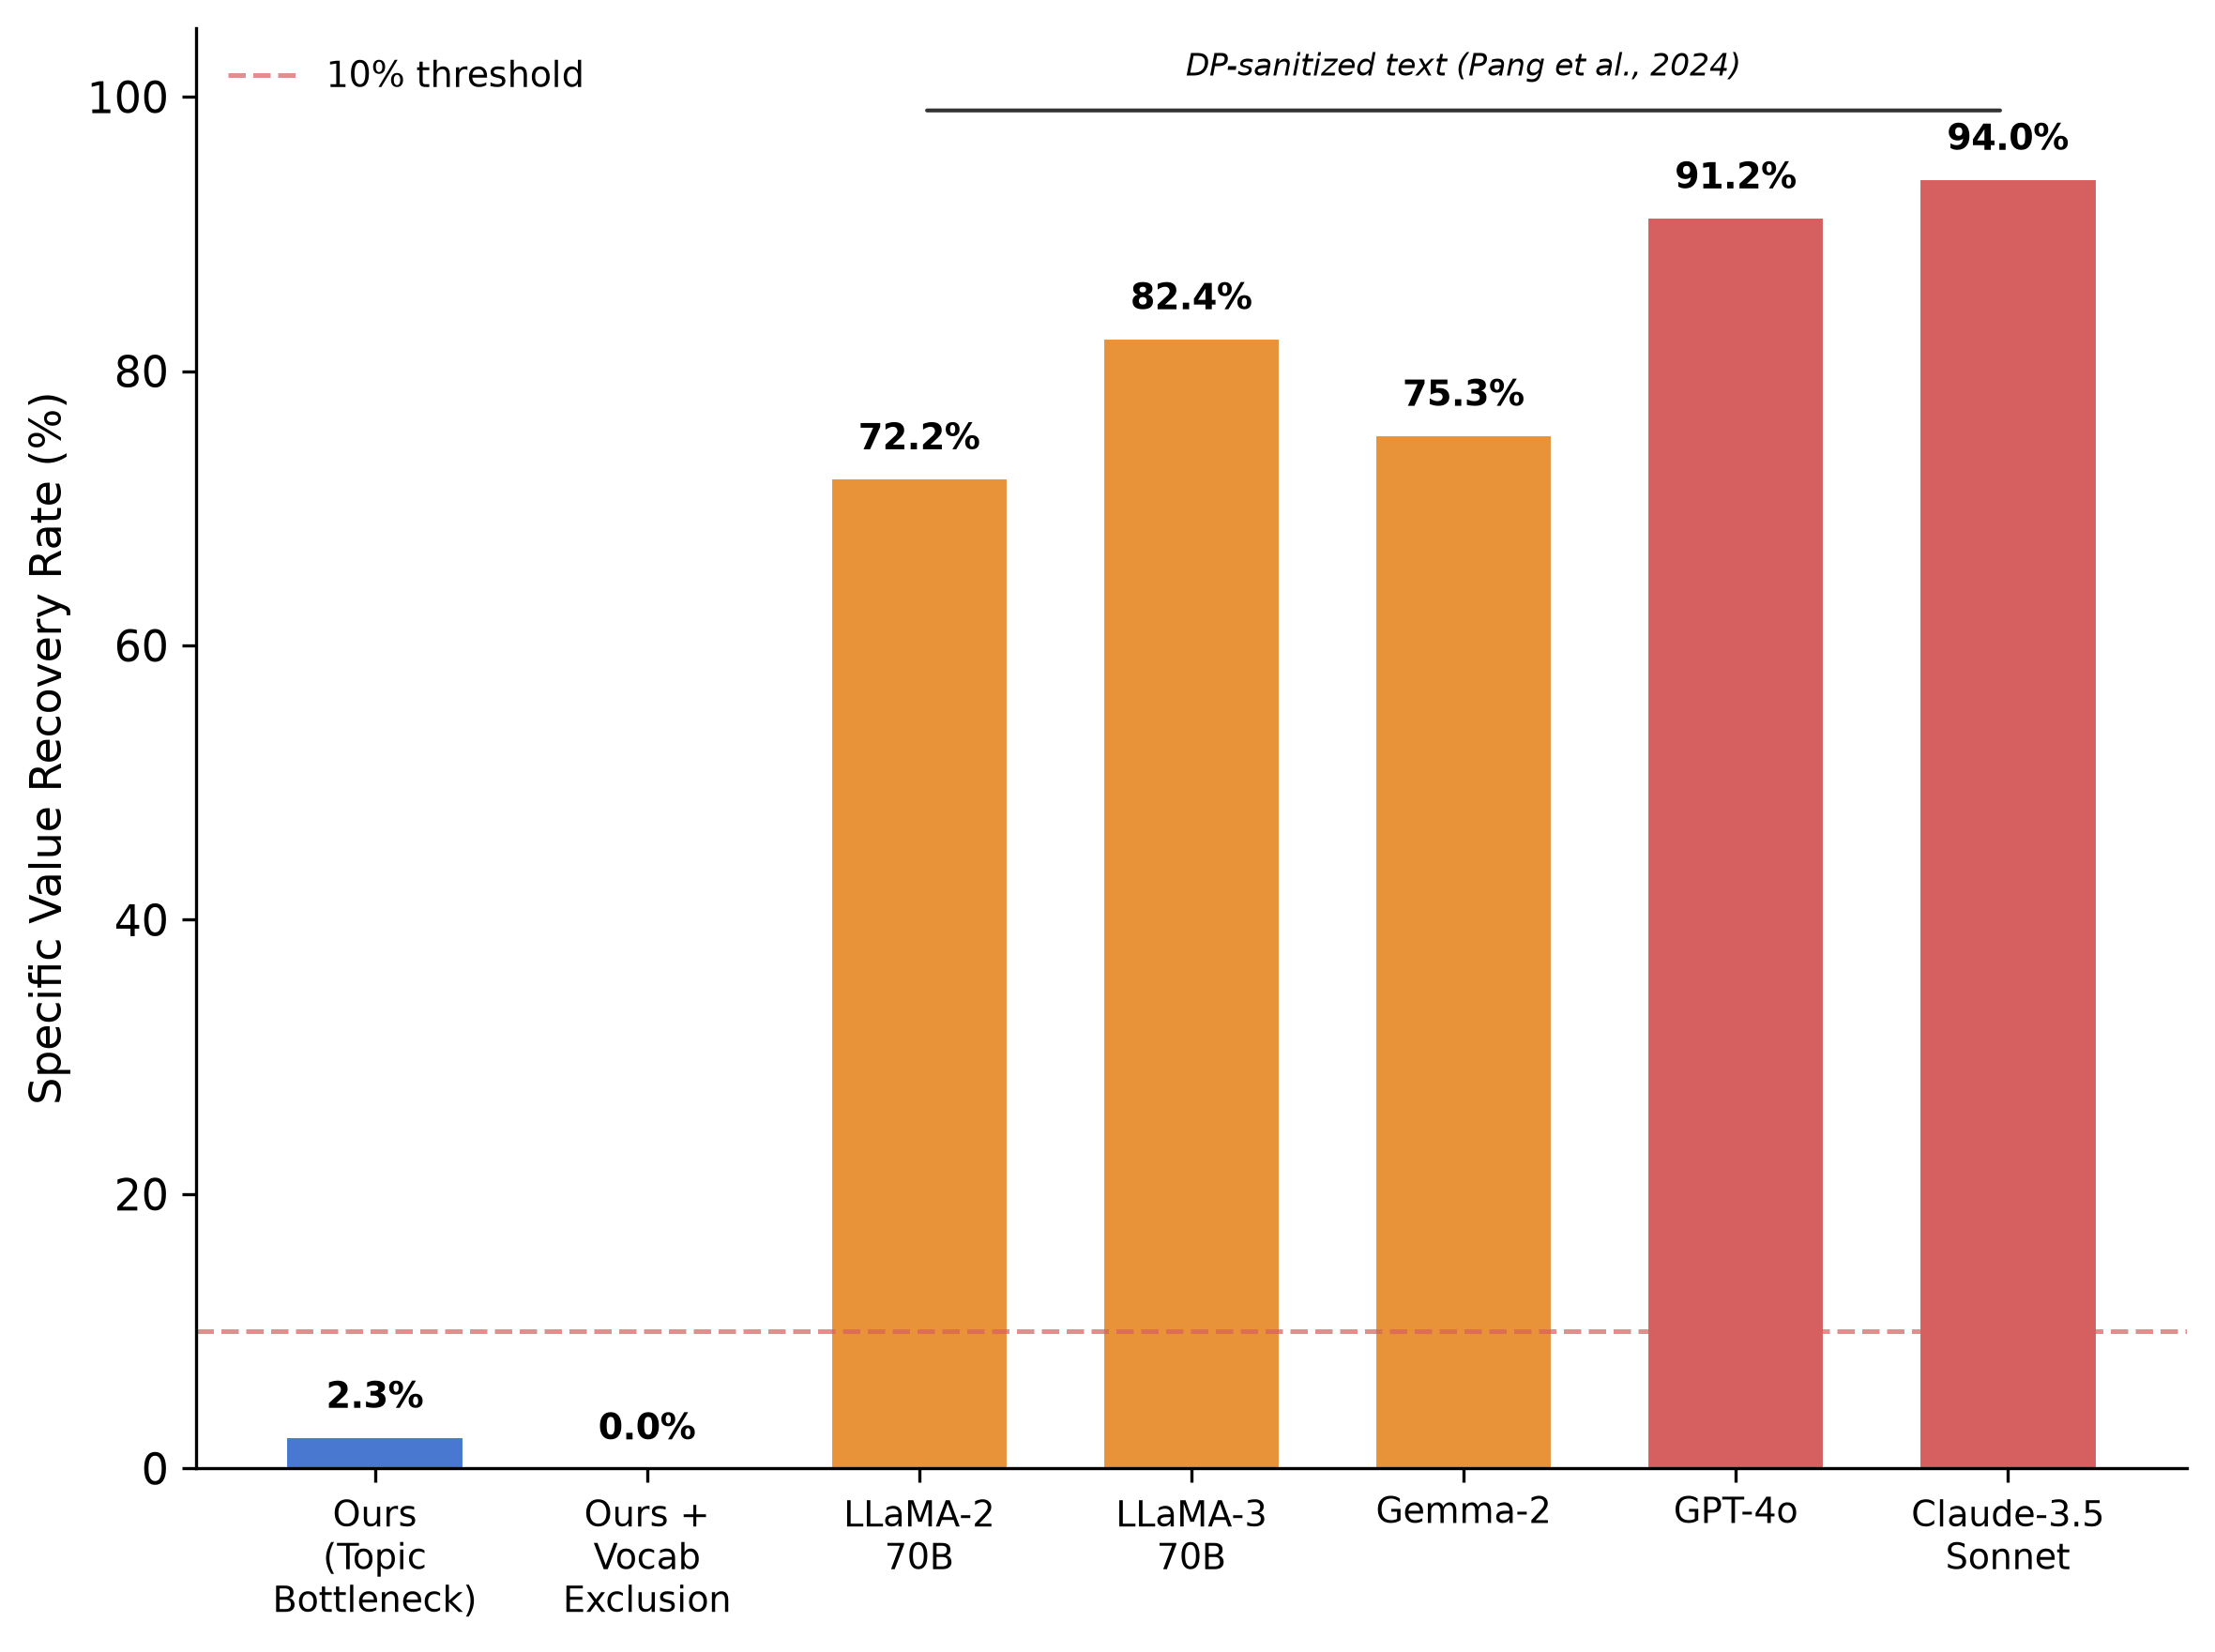
\includegraphics[width=\columnwidth]{fig_recovery_rate_comparison.png}
\caption{Specific value recovery rates for our topic-bottleneck pipeline compared with DP-sanitized text attacked by various LLMs (Pang et al., 2024). Our approach achieves 2.3\% recovery (0\% with vocabulary exclusion), compared to 72--94\% for differential privacy methods. The dashed red line indicates the 10\% acceptable recovery threshold.}
\label{fig:recovery}
\end{figure}

Domain recovery is high (90--94\%), indicating that adversaries can infer the general legal/contract domain from the proxy questions. This is expected and accepted by design: the topic structure is intentionally preserved. Situation scores are low (mean 0.254 for direct recovery, 0.266 for domain expert), indicating that adversaries can partially infer the \emph{type} of contractual situation but cannot identify the specific parties or terms.

\paragraph{Vocabulary exclusion ablation.} With vocabulary exclusion enabled, specific value recovery drops to \textbf{0.0\%}---perfect privacy---at the cost of quality degradation discussed in Section~\ref{sec:quality-results}. Figure~\ref{fig:scatter} shows the quality-privacy trade-off.

\begin{figure}[t]
\centering
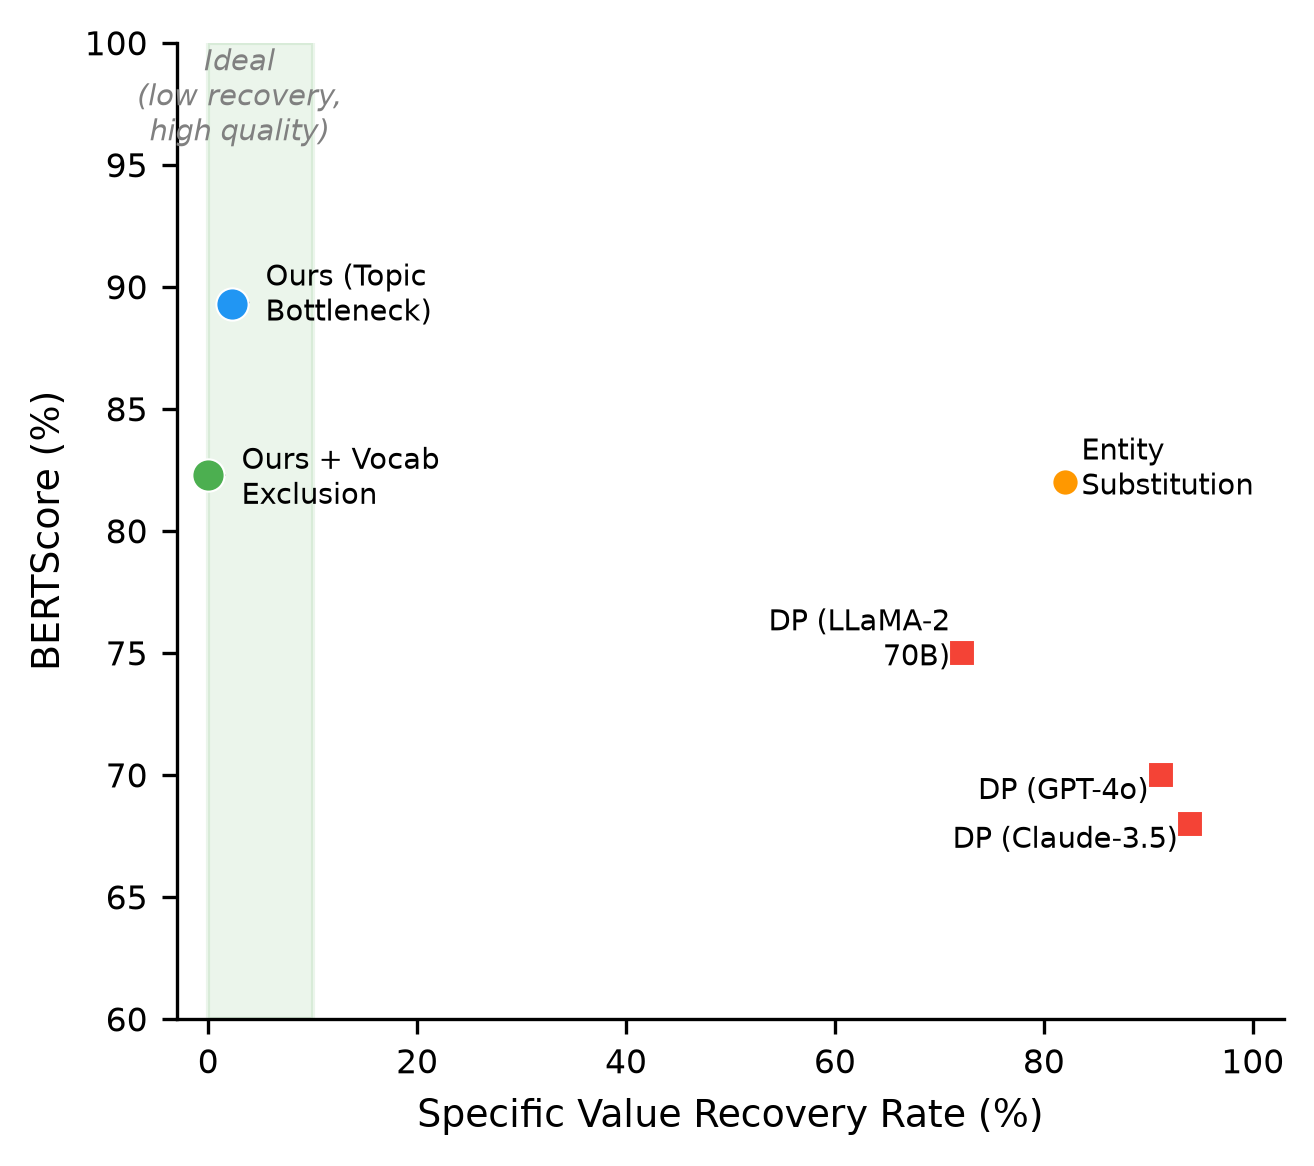
\includegraphics[width=\columnwidth]{fig_quality_privacy_scatter.png}
\caption{Quality-privacy trade-off across methods. The x-axis shows specific value recovery rate (lower is better for privacy) and the y-axis shows BERTScore F1 (higher is better for quality). Our pipeline and the entity substitution baseline are measured on CUAD; DP method recovery rates are from Pang et al.~\cite{pang2024} with quality values estimated from the literature (not measured on CUAD). The green-shaded area marks the target zone below 10\% recovery.}
\label{fig:scatter}
\end{figure}

\subsection{Quality: Answer Preservation}
\label{sec:quality-results}

Table~\ref{tab:quality} presents the answer quality metrics.

\begin{table}[h!]
\caption{Answer quality comparison (N=48). BERTScore F1 and semantic similarity are measured against the oracle (cloud LLM given the full S2 question).}
\label{tab:quality}
\small
\begin{tabular}{@{}lccc@{}}
\toprule
\textbf{Method} & \textbf{BERT F1} & \textbf{Sem.\ Sim.} & \textbf{Gold Ovl.} \\
\midrule
Oracle & 1.000 & 1.000 & --- \\
Local-only & 0.933 & 0.927 & 0.176 \\
Entity substitution & 0.820 & 0.581 & 0.021 \\
\textbf{Ours} & \textbf{0.893} & \textbf{0.853} & 0.225 \\
Ours + vocab exclusion & 0.823 & 0.413 & --- \\
\bottomrule
\end{tabular}
\end{table}

The pipeline preserves 89.3\% BERTScore F1 relative to the oracle, substantially outperforming the entity substitution baseline (82.0\% BERTScore, 58.1\% semantic similarity). The local-only baseline achieves higher BERTScore (93.3\%) because it has full access to the S2 question and can echo its content directly; however, it provides no cloud LLM reasoning capability, and its high surface similarity does not necessarily indicate superior answer utility---it reflects lexical overlap with the oracle answer rather than the application of specialized reasoning.

The pipeline produces answers that are on average 1.61$\times$ the length of oracle answers, consistent with a reasoning-based answer style rather than extractive span selection. Gold span overlap is low (22.5\%), confirming this interpretation.

\paragraph{Vocabulary exclusion quality cost.} Vocabulary exclusion reduces BERTScore F1 from 0.893 to 0.823 ($-$7.0 percentage points) and semantic similarity from 0.853 to 0.413 ($-$44.0 percentage points). The steep semantic similarity drop indicates that stripping topic vocabulary disrupts the S0 text's coherence enough to meaningfully degrade the cloud LLM's responses. This validates that vocabulary exclusion should be reserved for S3 (strictly confidential) data where even 2.3\% recovery is unacceptable.

\subsection{Task-Type Analysis}
\label{sec:task-results}

Table~\ref{tab:task} and Figure~\ref{fig:heatmap} present per-task-type results.

\begin{table}[t]
\caption{Performance by task type (n=12 per type, baseline configuration without vocabulary exclusion). 95\% confidence intervals in brackets.}
\label{tab:task}
\begin{tabular}{lcccc}
\toprule
\textbf{Task Type} & \textbf{BERT F1} & \textbf{Sem.\ Sim.} & \textbf{Gold Ovl.} & \textbf{Spec.\ Rec.} \\
\midrule
Framework & 0.890 & 0.814 & 0.083 & 0.000 \\
Compliance & 0.890 & 0.862 & 0.000 & 0.000 \\
Procedural & 0.887 & 0.866 & 0.167 & 0.000 \\
Entity-Spec. & 0.907 & 0.869 & 0.650 & 0.092 \\
\bottomrule
\end{tabular}
\end{table}

\begin{figure}[t]
\centering
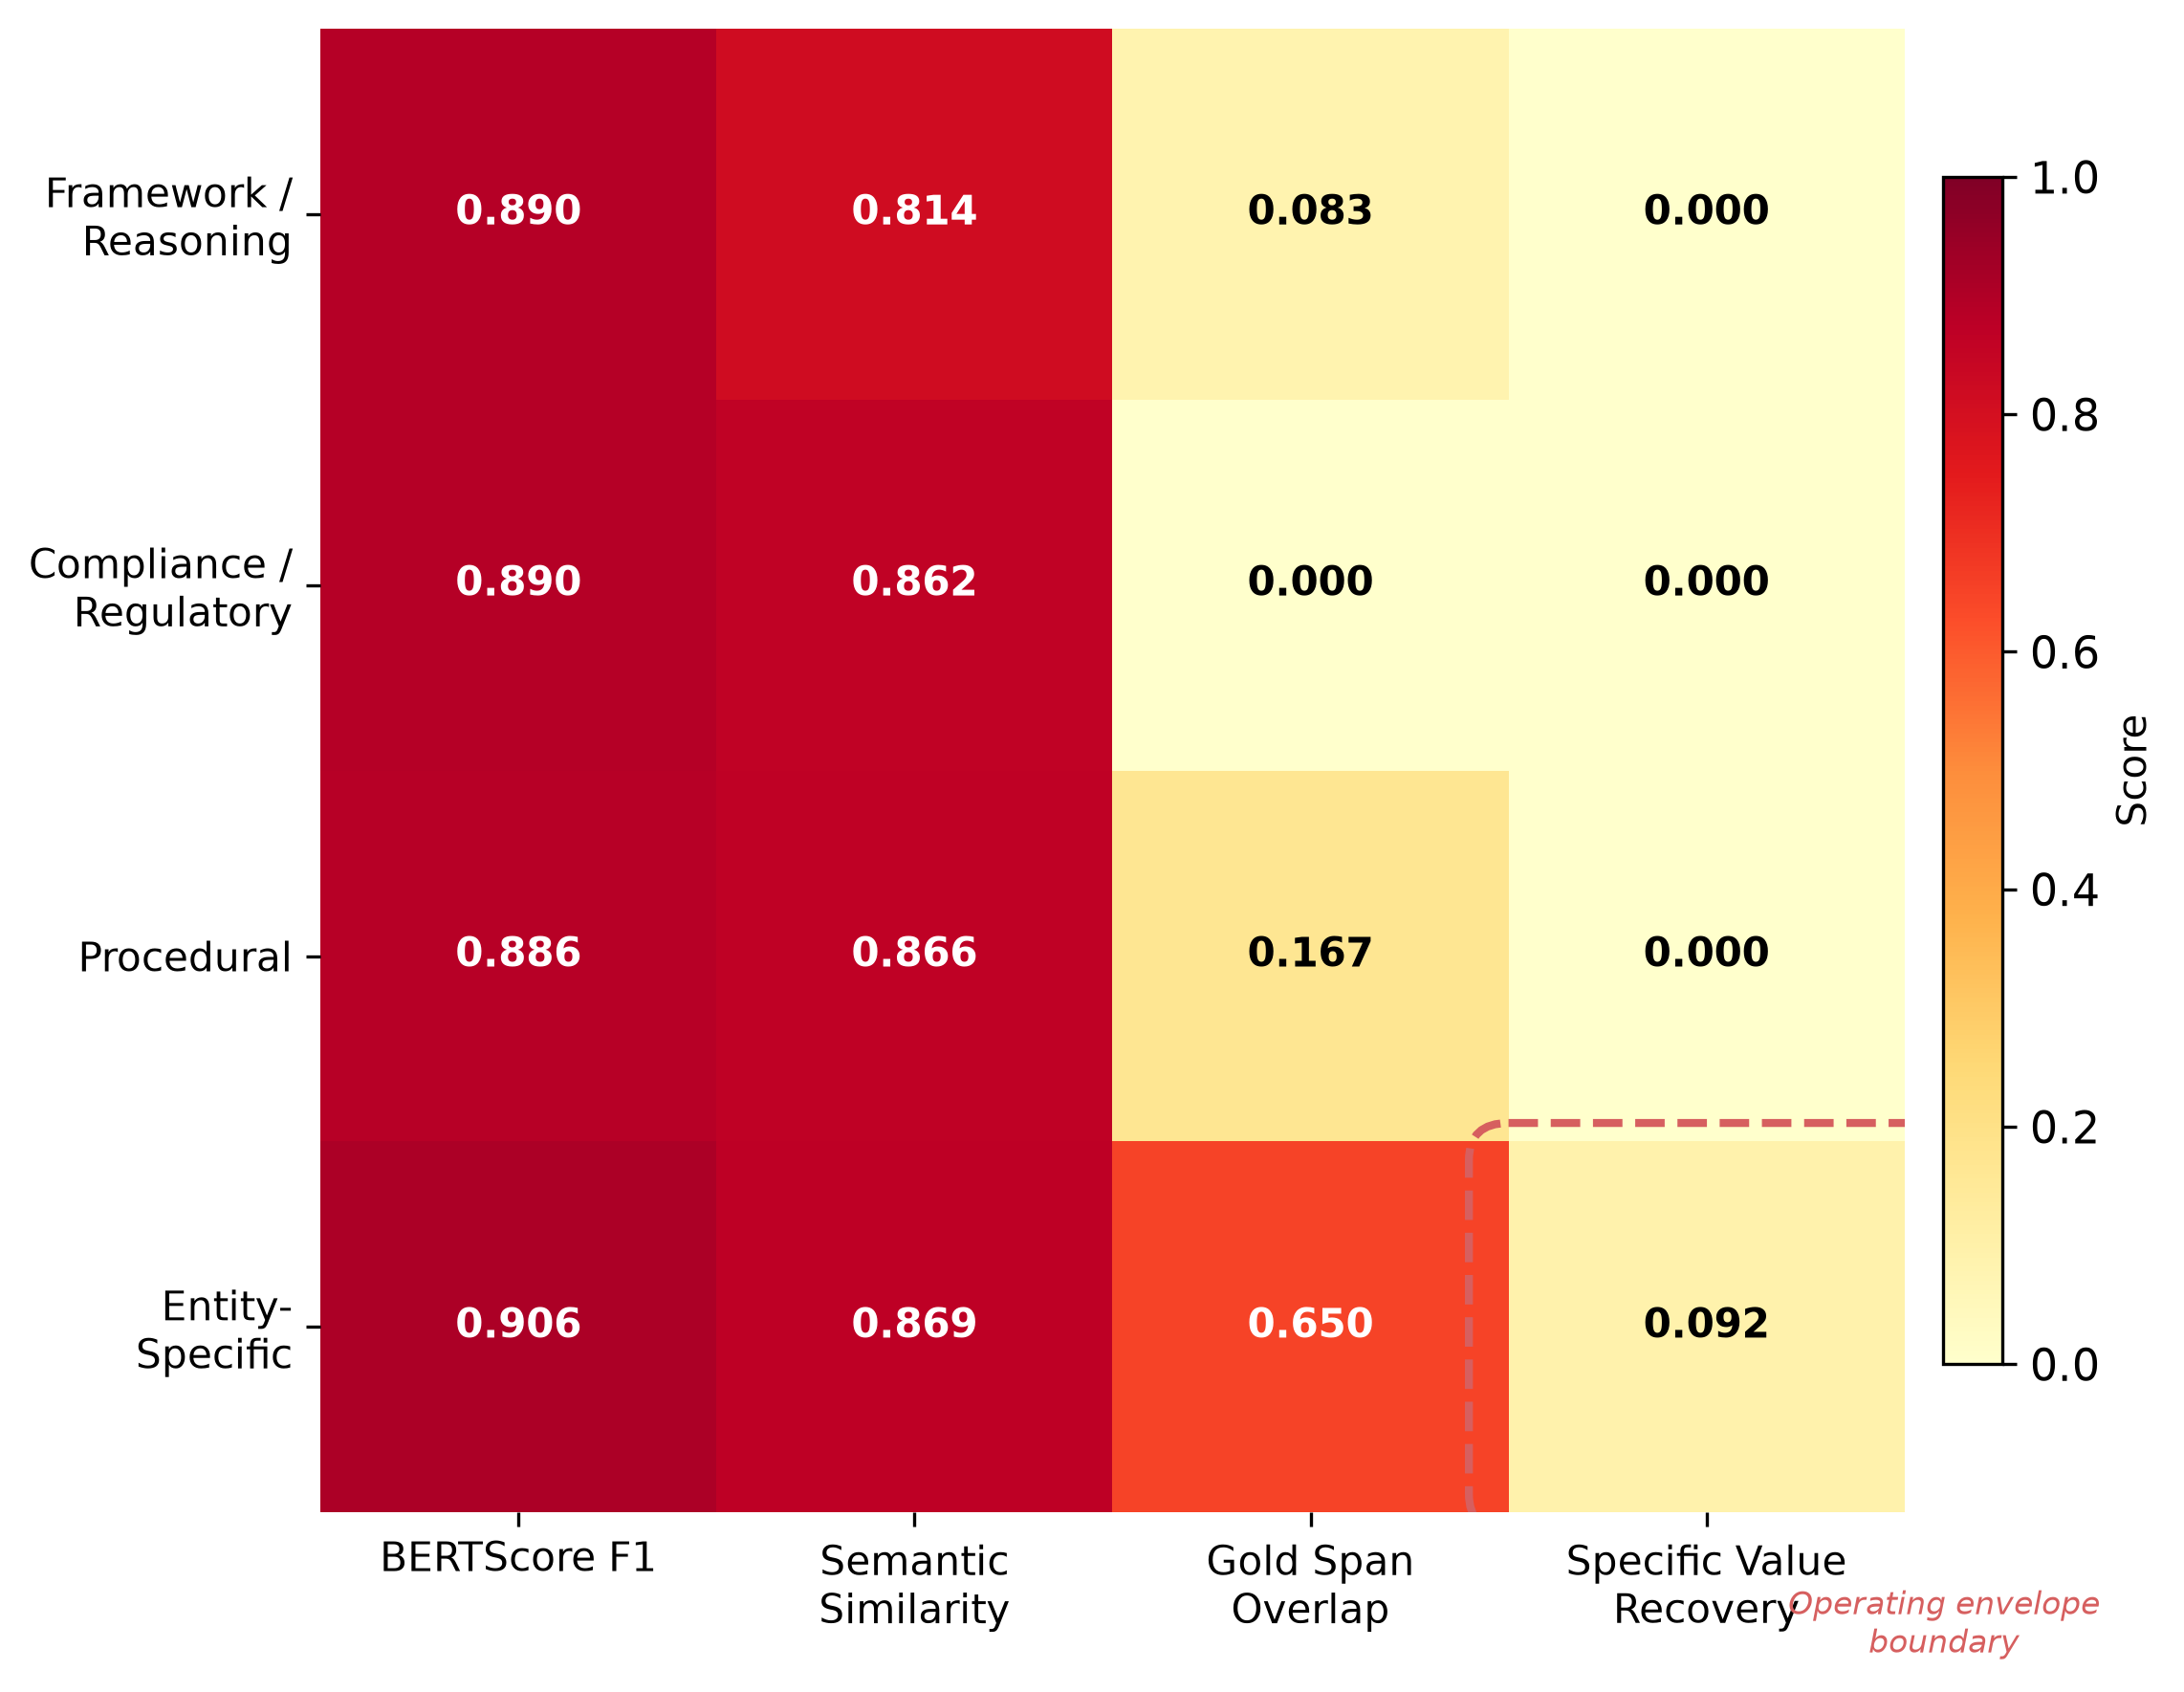
\includegraphics[width=\columnwidth]{fig_task_type_heatmap.png}
\caption{Performance metrics across four task types (n=12 each). Framework/reasoning, compliance, and procedural tasks achieve zero specific value recovery with strong BERTScore F1 (0.886--0.890). Entity-specific tasks show the expected quality-privacy trade-off with higher gold span overlap (0.65) and non-zero recovery (9.2\%). The dashed boundary highlights the operating envelope limit.}
\label{fig:heatmap}
\end{figure}

\paragraph{Operating envelope confirmed.} Framework/reasoning, compliance, and procedural tasks all achieve \textbf{zero specific value recovery} with strong BERTScore F1 (0.886--0.890). The pipeline operates well within its design envelope for these task types.

\paragraph{Entity-specific tasks.} Entity-specific queries show the highest gold span overlap (0.650) and the only non-zero specific value recovery (9.2\%, 95\% CI [0.000, 0.258]). The wide confidence interval---which includes zero---suggests this may be driven by a small number of outlier samples. We note one specific outlier (a document-name query about a restaurant chain contract) that achieved 100\% recovery on a single entity name. Entity-specific queries are the expected weakness: they require the sensitive specifics that the bottleneck intentionally strips.

\paragraph{Recovery case analysis.} Only 2 of 48 samples exhibited non-zero specific value recovery. In both cases, the ``recovered'' values were benign. Sample~1 (CUAD category: ``Parties''): the expert attacker partially guessed one party name out of five (10\% SVR); the proxy questions contained no identifying information, and the guess relied on domain knowledge rather than leaked data. Sample~2 (CUAD category: ``Document Name''): the gold answer was the contract type itself (``Sponsorship Agreement''), which the topic distribution necessarily preserves---the topic IS the sensitive value. Recovery was 100\% because the topic name matched the gold span exactly. Neither case involved recovery of financially sensitive information (deal values, competitive terms, dates). The 2.3\% aggregate recovery rate is driven entirely by edge cases where the CUAD annotation labels category-level metadata as the ``sensitive'' value, not by leakage of the entity names, monetary amounts, or temporal specifics that constitute genuine business sensitivity.

\paragraph{BERTScore anomaly.} Counterintuitively, entity-specific tasks achieve the \emph{highest} BERTScore F1 (0.907 vs.\ 0.887--0.890 for other types). This does not indicate superior performance. Rather, entity-specific CUAD categories (e.g., ``Parties,'' ``Document Name,'' ``Agreement Date'') elicit short, formulaic answers from both the pipeline and oracle---both produce similar legal boilerplate that overlaps lexically even when the pipeline fails to recover the specific entity. The high gold span overlap (0.650 vs.\ 0.000--0.167 for other types) confirms that these categories have concrete, extractable answer spans. BERTScore captures surface lexical similarity but not factual correctness; a human evaluation of answer utility would likely show the opposite ranking.

\paragraph{Bottleneck fidelity.} The three selected proxy questions achieve a mean maximum cosine similarity of 0.613 and mean coverage of 0.607 relative to the original S2 question, confirming that the bottleneck preserves approximately 61\% of the original query's semantic space---sufficient for topic-level reasoning but not for specific-value extraction.

%% ============================================================
%% SECTION 7: DISCUSSION
%% ============================================================
\section{Discussion}
\label{sec:discussion}

\subsection{Why the Information Bottleneck Works}
\label{sec:why-works}

The qualitative difference between our 2.3\% recovery rate and the 91--94\% rate for DP methods is not an incremental improvement---it reflects a fundamentally different privacy mechanism.

DP sanitization applies a many-to-many perturbation: each token is replaced with a noisy alternative drawn from a neighborhood in embedding space. The original token remains within the support of the perturbation distribution, and a sufficiently capable model can exploit training-data memorization to invert the perturbation. Entity substitution creates a one-to-one mapping that is straightforwardly invertible.

Topic extraction, by contrast, implements a many-to-one mapping. The space of sensitive queries that map to the same topic distribution, e.g.,
\[
\boldsymbol{\tau} = \bigl\{(\text{M\&A},\, 0.6),\; (\text{antitrust},\, 0.25),\; (\text{SaaS},\, 0.15)\bigr\}
\]
is combinatorially large: any company, any deal size, any market share, any timeline that involves M\&A with antitrust considerations in the SaaS sector maps to the same distribution. The mapping has no inverse function; reconstruction requires guessing from a space whose size grows exponentially with the number of possible specific values.

Table~\ref{tab:comparison} summarizes the key properties of our approach relative to the main competing paradigms.

\begin{table}[t]
\caption{Comparison of privacy-preserving LLM inference approaches. Recovery rates for DP methods are from Pang et al.~\cite{pang2024}; TEE and FHE overhead from the respective papers.}
\label{tab:comparison}
\begin{tabular}{lccc}
\toprule
\textbf{Approach} & \textbf{Recovery} & \textbf{Hardware} & \textbf{Deployable} \\
\midrule
Entity substitution & Invertible & None & Now \\
DP sanitization & 72--94\% & None & Now \\
Split inference & Variable & GPU & Partial \\
TEE (H100 CC) & Protected & H100 & Now \\
FHE/MPC & Protected & GPU+FHE & No \\
\textbf{Ours} & \textbf{2.3\%} & \textbf{None} & \textbf{Now} \\
Ours + vocab excl. & 0.0\% & None & Now \\
\bottomrule
\end{tabular}
\end{table}

\subsection{Operating Envelope and Deployment Guidance}
\label{sec:envelope}

The task-type analysis establishes a clear operating envelope:

\begin{itemize}
\item \textbf{Strong fit:} Framework/reasoning, compliance/regulatory, procedural queries. These task types together represent an estimated 60--70\% of enterprise LLM use cases. The pipeline provides strong privacy (zero recovery) with high quality (BERTScore $\geq$ 0.886).
\item \textbf{Weak fit:} Entity-specific and quantitative queries. These require the sensitive specifics that the bottleneck strips by design. They should be routed to local models or TEE-based inference.
\end{itemize}

A system that reliably handles 60--70\% of enterprise LLM use cases with strong privacy properties---and \emph{knows its limits} for the remaining 30--40\%---is more deployable than one that claims universal coverage. We recommend a graduated deployment model: S1 data uses the standard topic bottleneck; S2 data uses the bottleneck with vocabulary exclusion as an optional hardening step; S3 data uses the bottleneck with mandatory vocabulary exclusion.

The vocabulary exclusion trade-off is stark: perfect privacy (0\% recovery) at a steep quality cost (semantic similarity drops 44 percentage points). We recommend it only for S3 scenarios where even the 2.3\% baseline recovery rate is unacceptable. For S1 and S2 data, the standard bottleneck provides sufficient privacy with substantially better quality.

\subsection{Limitations}
\label{sec:limitations}

\paragraph{Single dataset.} Our evaluation uses only CUAD (legal contracts). Generalization to healthcare, finance, internal process, and other S2/S3 domains is untested. The privacy properties should transfer (the bottleneck mechanism is domain-independent), but quality preservation may vary with domain.

\paragraph{Small sample size.} N=48 (12 per task type) yields wide confidence intervals, particularly for entity-specific recovery where the CI includes zero. Larger-scale evaluation is needed to establish precise recovery rates by task type.

\paragraph{Absence fingerprint attack not evaluated.} We characterize the vulnerability theoretically (Section~\ref{sec:vocab-exclusion}) and propose four mitigations, but we did not empirically test the attack or the mitigations. The fingerprint vulnerability may partially undermine the privacy gains of vocabulary exclusion.

\paragraph{Untested attack variants.} The in-context learning (ICL) attack---where the adversary is given example (S2, S0) pairs---was not evaluated. Session-level aggregation attacks, where an adversary correlates multiple queries from the same user, were not evaluated. Both could reveal more information than single-query attacks.

\paragraph{Local model capacity.} Phi-3 (3.8B parameters) is a capable but not state-of-the-art local model. The synthesis step's quality is bounded by the local model's ability to apply external reasoning frameworks to specific data. Larger local models (e.g., Llama-3 70B) may yield different quality-privacy trade-offs.

\paragraph{Latency.} The pipeline requires approximately 39 seconds per query (31 minutes for 48 samples), dominated by cloud answering latency. This may be impractical for interactive use cases without optimization.

\paragraph{Ethical considerations.} Our reconstruction attacks use only public benchmark data (CUAD contracts) and do not involve real personal or enterprise data. The attack methodology demonstrates vulnerabilities in existing privacy methods; responsible disclosure norms are followed. The pipeline itself is designed to protect sensitive data, and our evaluation of its limitations (entity-specific leakage, absence fingerprint) is intended to prevent premature deployment in scenarios where these weaknesses are material.

%% ============================================================
%% SECTION 8: CONCLUSION
%% ============================================================
\section{Conclusion}
\label{sec:conclusion}

\subsection{Summary}
\label{sec:summary}

We introduced topic-bottleneck query reformulation, a pipeline for privacy-preserving cloud LLM inference that routes sensitive queries through an irreversible many-to-one information bottleneck. Unlike entity substitution and DP methods---from which modern LLMs recover 72--94\% of original content---our pipeline achieves 2.3\% specific value recovery while preserving 89.3\% BERTScore F1 quality. An optional vocabulary exclusion layer achieves 0\% recovery at the cost of a 7-percentage-point quality reduction. We characterized the operating envelope across four task types, demonstrating zero recovery for framework, compliance, and procedural queries and identifying entity-specific queries as the design boundary.

\subsection{Future Work}
\label{sec:future}

Several directions merit investigation. First, multi-domain evaluation beyond legal contracts---healthcare, finance, and internal process scenarios---would test generalization. Second, empirical evaluation of the absence fingerprint attack and its four proposed mitigations (Section~\ref{sec:vocab-exclusion}), particularly generation-time avoidance, is needed to validate the vocabulary exclusion variant. Third, the ICL attack variant and session-level aggregation attacks should be evaluated to characterize multi-query privacy. Fourth, larger local models may shift the quality-privacy Pareto frontier. Fifth, latency optimization---batched proxy generation, cached topic distributions, speculative generation---could make the pipeline suitable for interactive use. Finally, a formal privacy guarantee connecting the topic compression to information-theoretic bounds (e.g., bounding the mutual information between the topic distribution and any specific sensitive value) would strengthen the theoretical foundation.

\clearpage
\bibliographystyle{ACM-Reference-Format}
\bibliography{refs}

\appendix

\section{Bottleneck Fidelity Metrics}
\label{app:fidelity}

Table~\ref{tab:fidelity} reports the bottleneck fidelity metrics measuring how well the three selected proxy questions span the semantic space of the original S2 question.

\begin{table}[h]
\caption{Bottleneck fidelity metrics (N=48).}
\label{tab:fidelity}
\begin{tabular}{lc}
\toprule
\textbf{Metric} & \textbf{Mean} \\
\midrule
Max similarity (best proxy vs.\ original) & 0.613 \\
Mean similarity (avg proxy vs.\ original) & 0.496 \\
Coverage (semantic coverage of topic space) & 0.607 \\
\bottomrule
\end{tabular}
\end{table}

\section{Attack Variant Details}
\label{app:attacks}

Table~\ref{tab:attack-detail} provides detailed metrics for each attack variant.

\begin{table}[h]
\caption{Detailed attack variant results (N=48).}
\label{tab:attack-detail}
\small
\begin{tabular}{@{}lccc@{}}
\toprule
\textbf{Attack} & \textbf{Domain Rec.} & \textbf{Sit.\ Score} & \textbf{Value Rec.} \\
\midrule
Direct Recovery & 89.6\% & 0.254 & 2.1\% \\
In-Context Learning & 93.8\% & --- & 2.1\% \\
Domain Expert & 93.8\% & 0.266 & 2.5\% \\
Absence Fingerprint & \multicolumn{3}{c}{Not evaluated (see Section~\ref{sec:vocab-exclusion})} \\
\bottomrule
\end{tabular}
\end{table}

\section{Pipeline Timing}
\label{app:timing}

Total pipeline time for 48~samples was 1868.28 seconds (31.1 minutes), averaging 38.92 seconds per sample. Cloud answering latency (Azure OpenAI GPT-4o) contributes approximately 20--25 seconds per sample; local LLM steps (Phi-3) contribute approximately 10--15 seconds per sample.

\section{Task-Type Confidence Intervals}
\label{app:ci}

Table~\ref{tab:ci} provides the full 95\% confidence intervals for all task types.

\begin{table*}[h]
\caption{Full results by task type with 95\% confidence intervals (n=12 per type).}
\label{tab:ci}
\begin{tabular}{lcccc}
\toprule
\textbf{Task Type} & \textbf{BERTScore F1} & \textbf{Semantic Similarity} & \textbf{Gold Span Overlap} & \textbf{Specific Value Recovery} \\
\midrule
Framework/Reasoning & 0.890 [0.880, 0.900] & 0.814 [0.754, 0.866] & 0.083 [0.000, 0.250] & 0.000 [0.000, 0.000] \\
Compliance/Regulatory & 0.890 [0.878, 0.902] & 0.862 [0.822, 0.901] & 0.000 [0.000, 0.000] & 0.000 [0.000, 0.000] \\
Procedural & 0.887 [0.877, 0.897] & 0.866 [0.835, 0.899] & 0.167 [0.000, 0.333] & 0.000 [0.000, 0.000] \\
Entity-Specific & 0.907 [0.893, 0.925] & 0.869 [0.829, 0.906] & 0.650 [0.383, 0.900] & 0.092 [0.000, 0.258] \\
\bottomrule
\end{tabular}
\end{table*}

\end{document}
